\documentclass[14pt,a4paper]{extarticle}

\usepackage{fontspec}
\usepackage{polyglossia}
\setdefaultlanguage{russian}
\setotherlanguage{english}
\setmainfont{Times New Roman}[Script=Latin]
\setmonofont{Liberation Mono}
\newfontfamily\cyrillicfont{Times New Roman}[Script=Cyrillic]
\newfontfamily\cyrillicfonttt{Liberation Mono}[Script=Cyrillic]

\usepackage{geometry}
\geometry{top=2cm,bottom=2cm,left=3cm,right=1.5cm}

\usepackage{setspace}
\onehalfspacing

\usepackage{amsmath,amssymb}
\usepackage{indentfirst}
\setlength{\parindent}{1.25cm}

\usepackage{booktabs}
\usepackage{array}
\usepackage{tabularx}
\usepackage{graphicx}
\graphicspath{{../results/}}

\usepackage{hyperref}
\hypersetup{
  colorlinks=true,
  linkcolor=black,
  citecolor=black,
  urlcolor=black,
  pdftitle={Курсовая работа},
  pdfauthor={Цыбин Е. А.}
}

% Section: CAPS, centered, bold, 16pt, no period after number.
% Page break is done by titlesec's pagebreak option so TOC records the
% correct page (the post-break one, where the heading actually lives).
\usepackage[pagestyles]{titlesec}
\titleformat{\section}
  {\centering\bfseries\fontsize{16}{19}\selectfont\MakeUppercase}
  {\thesection}{1em}{}
\titleformat{\subsection}
  {\bfseries\fontsize{14}{17}\selectfont}
  {\thesubsection}{0.6em}{}
\titlespacing*{\section}{0pt}{0pt}{18pt}
\titlespacing*{\subsection}{1.25cm}{12pt}{12pt}
\newcommand{\sectionbreak}{\clearpage}

% Pagestyle: page number bottom-centered
\usepackage{fancyhdr}
\pagestyle{fancy}
\fancyhf{}
\fancyfoot[C]{\thepage}
\renewcommand{\headrulewidth}{0pt}

\newcommand{\definition}[2]{\par\noindent\textbf{Определение #1.} #2\par}
\newcommand{\theorem}[2]{\par\noindent\textbf{Теорема #1.} \emph{#2}\par}
\newcommand{\remark}[2]{\par\noindent\textbf{Замечание #1.} #2\par}

% Figure caption helpers
\usepackage{caption}
\captionsetup[figure]{name=Рисунок,labelsep=space,font={bf,small},justification=centering,skip=4pt}
\captionsetup[table]{name=Таблица,labelsep=space,font={bf,small},justification=centering,position=bottom,skip=4pt}

\begin{document}

% ===========================================================================
% Стр. 1. Титульный лист (без номера)
% ===========================================================================
\thispagestyle{empty}
\begin{center}
\textbf{МИНИСТЕРСТВО ОБРАЗОВАНИЯ РЕСПУБЛИКИ БЕЛАРУСЬ}\\[2pt]
Учреждение образования\\
\textbf{«Гродненский государственный университет имени Янки Купалы»}\\[2pt]
Факультет математики и информатики\\
Кафедра системного программирования и компьютерной безопасности

\vspace{3cm}

\textbf{ЦЫБИН ЕГОР АЛЕКСЕЕВИЧ}

\vspace{1.2cm}

\textbf{Анализ графа сетевого взаимодействия пользователей для выявления лидеров мнений и изолированных групп методами выделения сообществ и графовых нейронных сетей}

\vspace{1.2cm}

Курсовой проект по учебной дисциплине\\
«Машинное обучение и нейронные сети»\\
студента 3 курса специальности\\
6-05-0533-12 «Кибербезопасность»
\end{center}

\vspace{2.5cm}
\begin{flushright}
\begin{minipage}{0.55\textwidth}
Научный руководитель\\
Кадан Александр Михайлович,\\
заведующий кафедрой\\
системного программирования и компьютерной безопасности,\\
кандидат технических наук, доцент
\end{minipage}
\end{flushright}

\vfill
\begin{center}
Гродно 2026
\end{center}

% ===========================================================================
% Стр. 2. РЕФЕРАТ (русский)
% ===========================================================================
\newpage
\setcounter{page}{2}
\begin{center}\textbf{РЕФЕРАТ}\end{center}
\vspace{6pt}

Курсовой проект: 28 c., 3 рис., 7 табл., 19 источников.

\medskip
\noindent АНАЛИЗ ГРАФОВ, ВЫДЕЛЕНИЕ СООБЩЕСТВ, СОЦИОМЕТРИЯ, МОДУЛЯРНОСТЬ, АЛГОРИТМ ЛУВЕНА, АЛГОРИТМ ЛЕЙДЕНА, ГРАФОВЫЕ НЕЙРОННЫЕ СЕТИ, GCN, GRAPHSAGE, ЛИДЕРЫ МНЕНИЙ, ЦЕНТРАЛЬНОСТЬ.

\medskip
\textbf{Объект исследования:} графы сетевого взаимодействия пользователей в социальных сетях.

\textbf{Предмет исследования:} алгоритмы выделения сообществ, метрики центральности и графовые нейронные сети в задачах социометрии.

\textbf{Цель работы:} изучить методы анализа графа сетевого взаимодействия пользователей и эмпирически сравнить классические алгоритмы выделения сообществ и графовые нейронные сети в задаче выявления лидеров мнений и изолированных групп.

\textbf{Методы исследования:} теоретико-графовое моделирование, статистический анализ, эмпирический бенчмарк, машинное обучение на графах.

\textbf{Исследования и разработки:} исторический обзор от социограмм Морено \cite{moreno1934} до современных GNN; формализация задачи разбиения графа; описание алгоритмов Louvain \cite{blondel2008}, Leiden \cite{traag2019}, Label Propagation \cite{raghavan2007}, Girvan-Newman \cite{girvan2002}, Walktrap \cite{pons2006} и сетей GCN \cite{kipf2017} и GraphSAGE \cite{hamilton2017}; реализация модуля бенчмарка с метриками NMI, AMI, ARI, модулярности и точности; обучение GNN с разделением вершин на обучающую, валидационную и тестовую выборки и чекпоинтами; эмпирическое сравнение на Karate, Dolphins, Football, email-Eu-core, ego-Facebook и DBLP \cite{snap}.

\textbf{Элементы научной новизны:} систематизация классических и нейросетевых методов выделения сообществ в едином интерфейсе $f \colon G \to \mathbb{Z}^n$; воспроизводимое сравнение восьми алгоритмов и двух GNN-архитектур на шести датасетах.

\textbf{Область возможного практического применения:} анализ социальных сетей, выявление сообществ и лидеров мнений, обнаружение слабосвязанных групп, рекомендательные системы.

\medskip
Автор работы подтверждает, что приведённый в курсовом проекте расчётно-аналитический материал правильно и объективно отражает состояние исследуемого процесса, а все заимствованные из литературных и других источников теоретические, методологические и методические положения и концепции сопровождаются ссылками на их авторов.

% ===========================================================================
% Стр. 3. SUMMARY (английский)
% ===========================================================================
\newpage
\begin{english}
\begin{center}\textbf{SUMMARY}\end{center}
\vspace{6pt}

Course project: 28 pp, 3 fig, 7 tbl, 19 ref.

\medskip
\noindent GRAPH ANALYSIS, COMMUNITY DETECTION, SOCIOMETRY, MODULARITY, LOUVAIN ALGORITHM, LEIDEN ALGORITHM, GRAPH NEURAL NETWORKS, GCN, GraphSAGE, OPINION LEADERS, CENTRALITY.

\medskip
\textbf{The object of the research:} graphs of user communication in social networks.

\textbf{The subject of the research:} community detection algorithms, centrality measures and graph neural networks applied to sociometric tasks.

\textbf{The research objective:} to study methods of social graph analysis and empirically compare classical community detection algorithms with graph neural networks for the task of opinion-leader and isolated-group identification.

\textbf{Research methods:} graph-theoretic modelling, statistical analysis, empirical benchmarking, machine learning on graphs.

\textbf{Research and developments:} a historical review from Moreno's sociograms to modern GNNs; a formal description of graph partitioning; specification of Louvain, Leiden, Label Propagation, Girvan-Newman, Walktrap and GCN/GraphSAGE; a benchmark harness with NMI, AMI, ARI, modularity and best-permutation accuracy; GNN training with обучающая/валидационная/тестовая выборки split and model checkpointing; empirical comparison on Karate, Dolphins, Football, email-Eu-core, ego-Facebook and DBLP.

\textbf{Elements of scientific novelty:} unification of classical and neural community detection methods under a single interface $f \colon G \to \mathbb{Z}^n$; reproducible comparison of eight algorithms and two GNN architectures on six datasets.

\textbf{The field of possible practical use:} social network analysis, community and opinion-leader detection, weakly-connected group identification, recommender systems.
\end{english}

% ===========================================================================
% Стр. 4. СОДЕРЖАНИЕ
% ===========================================================================
\newpage
\renewcommand{\contentsname}{\hfill\textbf{СОДЕРЖАНИЕ}\hfill}
\tableofcontents

% ===========================================================================
% ВВЕДЕНИЕ
% ===========================================================================
\section*{ВВЕДЕНИЕ}
\addcontentsline{toc}{section}{ВВЕДЕНИЕ}

\textbf{Актуальность темы.} Современная коммуникация всё чаще опосредуется цифровыми социальными сетями: пользователи обмениваются сообщениями, образуют сообщества, формируют общественное мнение через лидеров и оказываются в изолированных группах. Объёмы накапливаемых данных таковы, что ручной социометрический анализ невозможен, а традиционные опросные методы не масштабируются. Задача автоматического выявления лидеров мнений и изолированных групп критична для рекомендательных систем, маркетинга, обнаружения координированной активности и понимания политической поляризации. При этом методы анализа графов прошли существенную эволюцию- от качественных социограмм Морено \cite{moreno1934} до современных графовых нейронных сетей \cite{kipf2017,hamilton2017}- и выбор между ними на практике далеко не очевиден.

\textbf{Практическая значимость} работы состоит в построении воспроизводимого модуля сравнения восьми классических алгоритмов выделения сообществ и двух графовых нейросетевых архитектур на эталонных и реальных датасетах. Полученные результаты позволяют обоснованно выбирать алгоритм в зависимости от размера графа, числа сообществ и наличия частичной разметки.

\textbf{Степень изученности.} Задача выделения сообществ изучается с 1970-х годов: классический датасет Захари \cite{zachary1977}, модулярность Ньюмана \cite{girvan2002}, алгоритмы Louvain \cite{blondel2008} и Leiden \cite{traag2019}, методы случайных блужданий Walktrap \cite{pons2006}. Современный этап представлен графовыми нейронными сетями GCN \cite{kipf2017} и GraphSAGE \cite{hamilton2017}, развиваемыми компаниями Google, Meta, Stanford SNAP \cite{snap} и др.

\textbf{Объект исследования}- графы сетевого взаимодействия пользователей в социальных сетях.

\textbf{Предмет исследования}- алгоритмы выделения сообществ, метрики центральности и графовые нейронные сети в задачах социометрии.

\textbf{Цель работы}- изучить методы анализа графа сетевого взаимодействия пользователей и эмпирически сравнить классические алгоритмы выделения сообществ и графовые нейронные сети в задаче выявления лидеров мнений и изолированных групп.

\textbf{Задачи работы:}
\begin{enumerate}
\item Изучить актуальность темы, проследить историю развития методов и проанализировать литературу.
\item Дать строгое математическое описание моделей графа, алгоритмов выделения сообществ, метрик центральности и нейросетевых архитектур GCN и GraphSAGE.
\item Провести эмпирическое сравнение методов на шести датасетах, проинтерпретировать полученные результаты.
\end{enumerate}

\textbf{Методы исследования:} теоретико-графовое моделирование, статистический анализ структурных характеристик графа, эмпирический бенчмарк алгоритмов, обучение графовых нейронных сетей.

\textbf{Структура работы.} Работа состоит из введения, трёх глав, заключения и списка использованных источников. Первая глава посвящена актуальности темы, истории вопроса и обзору литературы; вторая- теоретическому материалу; третья- практической реализации и эмпирическим результатам.

% ===========================================================================
% ГЛАВА 1
% ===========================================================================
\section{Актуальность темы, исторический обзор и обзор литературы}

\subsection{Актуальность задачи социометрии в условиях цифровых социальных сетей}

Социометрия как область знания зарождается в 1930-х годах в работах Я.~Морено \cite{moreno1934}, предложившего изображать межличностные отношения в виде графа. С появлением цифровых социальных сетей (Facebook, ВКонтакте, Twitter, Telegram) объём социометрических данных вырос на много порядков: типичная социальная сеть содержит миллионы вершин и миллиарды рёбер. Это сделало невозможным ручной анализ и потребовало автоматических алгоритмических методов.

Задача \emph{выявления лидеров мнений} имеет прямое практическое значение: лидеры- это узлы, чьё мнение быстрее всего распространяется по сети, поэтому маркетинг и информационные кампании ориентируются именно на них. Задача \emph{выявления изолированных групп}- обнаружение слабосвязанных подсообществ- важна для рекомендательных систем (изолированные пользователи получают плохие рекомендации), а также для обнаружения координированной дезинформации (изолированные «эхо-камеры»).

Графовое представление позволяет свести обе задачи к строгим математическим конструкциям. Пусть $G = (V, E)$- неориентированный граф взаимодействий, $|V| = n$, $|E| = m$. Тогда:
\begin{itemize}
\item лидеры мнений- узлы с наибольшими значениями метрик центральности (степенной, betweenness, closeness, eigenvector, PageRank);
\item изолированные группы- подмножества $S \subseteq V$ с малым conductance $\varphi(S) = |\partial S|/\min(\operatorname{vol}(S), \operatorname{vol}(V \setminus S))$.
\end{itemize}

\subsection{Историческая справка}

Идея графового представления социальных связей восходит к работе Я.~Морено «Who Shall Survive?» \cite{moreno1934}. Морено ввёл понятие \emph{социограммы} и стал применять её для анализа малых групп. Однако вплоть до 1950-х годов аппарат оставался качественным: социограммы рисовались вручную, формальных метрик не было.

Принципиальный сдвиг произошёл с публикацией П.~Эрдёшем и А.~Реньи серии работ о случайных графах \cite{erdos1959}. Модель $G(n, p)$ впервые позволила говорить о структуре графа в строгих вероятностных терминах. В 1977 году В.~Захари \cite{zachary1977} опубликовал ставший каноническим датасет карате-клуба- 34 члена и 78 рёбер с известным историческим расколом, до сих пор используемый как первый бенчмарк новых алгоритмов.

На рубеже 1990-2000-х Д.~Уоттс и С.~Строгатц \cite{watts1998} и А.~Барабаши и Р.~Альберт \cite{barabasi1999} показали, что реальные сети одновременно демонстрируют высокую кластеризацию, малую среднюю длину пути и степенное распределение степеней. Это привело к появлению моделей малого мира (WS) и сетей с предпочтительным присоединением (BA).

Современная эпоха алгоритмического выделения сообществ начинается с работы М.~Гирвана и М.~Ньюмана \cite{girvan2002}, в которой была введена \emph{модулярность}. Прямая оптимизация модулярности оказалась NP-трудной \cite{brandes2008}, поэтому В.~Блондель и соавторы \cite{blondel2008} предложили жадный алгоритм Louvain. В 2007 году С.~Фортунато и М.~Бартелеми \cite{fortunato2007} показали фундаментальное ограничение модулярности- \emph{предел разрешения}. В 2019 году В.~Трааг и соавторы \cite{traag2019} устранили недостаток Louvain (несвязные сообщества), предложив алгоритм Leiden.

Параллельно развивались алгоритмы случайных блужданий: Walktrap \cite{pons2006}; и быстрые эвристики: Label Propagation \cite{raghavan2007}.

С 2017 года наступает эпоха графовых нейронных сетей. Т.~Кипф и М.~Веллинг \cite{kipf2017} предложили GCN на основе аппроксимации Чебышёва спектральной свёртки \cite{defferrard2016}. В том же году В.~Хэмилтон и соавторы \cite{hamilton2017} представили GraphSAGE с раздельным обучением представления узла и его соседей.

\subsection{Обзор литературы и сравнение подходов}

Анализ литературы показывает, что в настоящее время сосуществуют три основных семейства методов выделения сообществ.

\textbf{Алгоритмы оптимизации модулярности} (Louvain \cite{blondel2008}, Leiden \cite{traag2019}, Fast Greedy)- наиболее распространённые в практике. Их преимущества: высокая скорость, отсутствие необходимости в разметке, понятная интерпретация. Недостаток- предел разрешения \cite{fortunato2007}: невозможность обнаруживать сообщества размера менее $\sqrt{2m}$.

\textbf{Алгоритмы на случайных блужданиях} (Walktrap \cite{pons2006})- основаны на наблюдении, что блуждания «застревают» в плотных сообществах. 

\textbf{Графовые нейронные сети} (GCN \cite{kipf2017}, GraphSAGE \cite{hamilton2017})- обучаемые модели, использующие частичную разметку и матрицу признаков. Они превосходят классические методы при наличии разметки, но требуют размеченных данных, GPU-ресурсов и подвержены переобучению. Современные обзоры \cite{newman2010,diestel2017} рассматривают эти три семейства как взаимодополняющие.

Стандартными датасетами для сравнения остаются Karate \cite{zachary1977}, Dolphins, Football \cite{girvan2002} и большие графы из репозитория Stanford SNAP \cite{snap}. Стандартными метриками качества- NMI, AMI, ARI и модулярность.

% ===========================================================================
% ГЛАВА 2
% ===========================================================================
\section{Математическая модель социального графа и методов его анализа}

\subsection{Граф и его матричные представления}

\definition{2.1}{Неориентированным графом называется упорядоченная пара $G = (V, E)$, где $V$- конечное непустое множество вершин, а $E \subseteq \{\{u, v\} : u, v \in V,\, u \neq v\}$- множество рёбер.}

\definition{2.2}{Матрицей смежности графа $G$, $|V| = n$, называется симметричная матрица $A \in \{0, 1\}^{n \times n}$ с
\begin{equation}
A_{ij} =
\begin{cases}
1, & \{v_i, v_j\} \in E,\\
0, & \text{иначе.}
\end{cases}
\end{equation}}

\definition{2.3}{Степенью вершины $v$ называется $\deg(v) = \sum_j A_{vj}$. Степенной матрицей называется $D = \operatorname{diag}(\deg(v_1), \dots, \deg(v_n))$.}

\definition{2.4}{Лапласианом графа называется $L = D - A$. Нормализованным лапласианом- матрица
\begin{equation}
L_{\mathrm{sym}} = D^{-1/2} L\, D^{-1/2} = I - D^{-1/2} A\, D^{-1/2}.
\end{equation}}

\theorem{2.1}{Матрица $L$ симметрична и положительно полуопределена. Все её собственные значения неотрицательны: $0 = \lambda_1 \leq \lambda_2 \leq \dots \leq \lambda_n$. Кратность нулевого собственного значения равна числу связных компонент графа \cite{newman2010}.}

\subsection{Модели случайных графов и модулярность}

\definition{2.5 ($G(n, p)$, \cite{erdos1959})}{Случайным графом Эрдёша-Реньи называется граф на $n$ вершинах, в котором каждое из $C_n^2$ рёбер включается независимо с вероятностью $p$. Ожидаемое число рёбер: $\mathbb{E}|E| = p \cdot n(n-1)/2$.}

\definition{2.6 ($\mathrm{BA}(n, m)$, \cite{barabasi1999})}{Модель Барабаши-Альберт строит граф последовательным добавлением узлов; каждый новый узел соединяется с $m$ существующими с вероятностью, пропорциональной их степени:
\begin{equation}
\Pr(v_t \sim u) = \frac{\deg(u)}{\sum_{w} \deg(w)}.
\end{equation}
При $n \to \infty$ распределение степеней сходится к степенному $\Pr(\deg = k) \sim k^{-3}$.}

\definition{2.7 ($\mathrm{WS}(n, k, p)$, \cite{watts1998})}{Граф малого мира строится из $k$-регулярной кольцевой решётки путём независимой перепосадки каждого ребра с вероятностью $p$.}

\definition{2.8 (модулярность Ньюмана, \cite{girvan2002})}{Модулярностью разбиения $\sigma$ называется
\begin{equation}
Q(\sigma) = \frac{1}{2m} \sum_{i,j} \left[ A_{ij} - \frac{k_i k_j}{2m} \right] \delta(\sigma(i), \sigma(j)),
\label{eq:modularity}
\end{equation}
где $k_i = \deg(i)$, $m = |E|$, $\delta$- символ Кронекера.}

Значение $Q \in [-1/2, 1]$; $Q > 0.3$ считается признаком значимой модульной структуры. Прямая оптимизация $Q$ NP-трудна \cite{brandes2008}.

\remark{2.1 (предел разрешения, \cite{fortunato2007})}{Оптимизация $Q$ не способна обнаружить сообщества размера менее $\sqrt{2m}$.}

\subsection{Классические алгоритмы выделения сообществ}

Прямая максимизация модулярности (определение~2.8) является NP-трудной задачей~\cite{brandes2008}: число возможных разбиений $n$ вершин на непустые непересекающиеся подмножества (число Белла $B_n$) растёт быстрее экспоненциально, и перебор невозможен уже при $n \approx 30$. Поэтому все практические алгоритмы- эвристические; они отличаются тем, какую структуру поиска используют и какой функционал оптимизируют. Ниже описаны шесть наиболее распространённых методов.

\paragraph{2.3.1 Алгоритм Лувена~\cite{blondel2008}.} Жадный многоуровневый метод. Идея: вместо поиска глобального оптимума модулярности находить локально оптимальные перемещения отдельных вершин, а затем повторять процедуру на сжатом графе. Алгоритм состоит из двух фаз, которые рекурсивно повторяются.

\textit{Фаза~1 (локальное перемещение).} Изначально каждой вершине $v \in V$ присваивается собственное сообщество. Далее в произвольном порядке для каждой вершины рассматриваются все сообщества $c$ её соседей; вершина переносится в то сообщество, которое даёт наибольший положительный прирост модулярности
\begin{equation}
\Delta Q(v \to c) = \frac{\Sigma_{\mathrm{in}}^c + 2 k_{v,c}}{2m} - \left( \frac{\Sigma_{\mathrm{tot}}^c + k_v}{2m} \right)^2 - \left[ \frac{\Sigma_{\mathrm{in}}^c}{2m} - \left( \frac{\Sigma_{\mathrm{tot}}^c}{2m} \right)^2 - \left( \frac{k_v}{2m} \right)^2 \right],
\end{equation}
где $\Sigma_{\mathrm{in}}^c$- сумма весов рёбер внутри сообщества $c$, $\Sigma_{\mathrm{tot}}^c$- сумма степеней вершин $c$, $k_{v,c}$- сумма весов рёбер от $v$ к вершинам $c$. Если максимальный $\Delta Q \leq 0$, вершина остаётся на месте. Фаза~1 повторяется до тех пор, пока хотя бы одна вершина меняет сообщество.

\textit{Фаза~2 (агрегирование).} Каждое сообщество, найденное на фазе~1, заменяется одной супер-вершиной; рёбра внутри сообщества становятся петлёй с весом, равным удвоенной внутренней сумме; рёбра между разными сообществами объединяются во взвешенные рёбра между супер-вершинами. На полученном уменьшенном графе снова запускается фаза~1, и так далее- пока модулярность продолжает расти.

Эмпирическая сложность алгоритма $O(n \log n)$; на графах с миллионами вершин Лувен сходится за минуты. Его главный недостаток- возможность образования несвязных сообществ (вершина может «утянуть» с собой группу, разорвав исходное сообщество), что было устранено в алгоритме Лейдена.

\paragraph{2.3.2 Алгоритм Лейдена~\cite{traag2019}.} Прямое улучшение алгоритма Лувена, гарантирующее связность найденных сообществ. Между фазами~1 и~2 вводится дополнительная \textit{фаза уточнения}.

После фазы~1 для каждого найденного сообщества $C$ его вершины снова помещаются каждая в своё под-сообщество; затем запускается ограниченное локальное перемещение, в котором вершины могут переходить только в под-сообщества, целиком содержащиеся в $C$. В результате каждое исходное сообщество $C$ разбивается на одно или несколько связных компонент-сообществ. Авторами доказано~\cite{traag2019}, что все сообщества, найденные алгоритмом Лейдена, связны, и что при достаточном числе итераций алгоритм сходится к $\gamma$-плотному разбиению. По эмпирической сложности Лейден сопоставим с Лувеном.

\paragraph{2.3.3 Алгоритм распространения меток (Label Propagation)~\cite{raghavan2007}.} Сверх-быстрый алгоритм без целевого функционала. Идея: каждая вершина «голосует» меткой большинства своих соседей, и при многократном повторении такого голосования вершины одного плотного сообщества постепенно приходят к общей метке.

Изначально каждой вершине присваивается уникальная метка $\ell^{(0)}(v) = v$. На итерации $t$ для каждой вершины $v$ (в случайном порядке) вычисляется новая метка как наиболее частая среди меток её соседей на предыдущей итерации:
\begin{equation}
\ell^{(t)}(v) = \arg\max_{\ell} \bigl|\{u \in N(v) : \ell^{(t-1)}(u) = \ell\}\bigr|.
\end{equation}
При нескольких максимумах метка выбирается случайно. Алгоритм сходится, когда ни одна метка не меняется; итоговые группы одинаковых меток образуют сообщества. Сложность $O(m)$ на итерацию, число итераций обычно невелико- метод реально работает за почти линейное время.

Основной недостаток- неустойчивость и тенденция к коллапсу. На плотных графах с большим числом классов одна-две начальные метки начинают доминировать и поглощают остальные, что в пределе приводит к разбиению на одну компоненту ($\hat k = 1$, $\operatorname{NMI} = 0$). Это явление эмпирически наблюдается на датасете email-Eu-core (см. раздел~3.3).

\paragraph{2.3.4 Алгоритм Гирвана-Ньюмана~\cite{girvan2002}.} Один из первых алгоритмов выделения сообществ, основанный на иерархическом удалении «мостов»- рёбер, лежащих на наибольшем числе кратчайших путей.

\definition{2.9 (промежуточность ребра)}{Промежуточностью ребра $e$ называется
\begin{equation}
C_B(e) = \sum_{s \neq t} \frac{\sigma_{st}(e)}{\sigma_{st}},
\end{equation}
где $\sigma_{st}$- число кратчайших путей из $s$ в $t$, $\sigma_{st}(e)$- число таких путей, проходящих через $e$.}

Алгоритм работает следующим образом: (1) для всех рёбер вычисляется $C_B(e)$; (2) удаляется ребро с максимальным $C_B$; (3) пересчитываются $C_B$ для оставшихся рёбер; (4) шаги повторяются, пока остаются рёбра. На каждом шаге фиксируется текущее разбиение графа на связные компоненты, и среди всех таких разбиений выбирается то, что максимизирует модулярность $Q$.

Идея метода: мосты, соединяющие разные сообщества, лежат на пути от любой вершины одного сообщества к любой вершине другого, поэтому имеют непропорционально большую промежуточность. Алгоритм Брандеса вычисляет $C_B$ всех рёбер за $O(nm)$, и таких подсчётов нужно $O(m)$, что даёт общую сложность $O(nm^2)$. На графах с $n > 1000$ метод практически неприменим, но на малых графах (Karate, Dolphins) даёт качественные разбиения.

\paragraph{2.3.5 Алгоритм Walktrap~\cite{pons2006}.} Иерархический алгоритм, использующий близость вершин в смысле случайных блужданий.

Определяется матрица переходов $P = D^{-1} A$. После $t$ шагов вероятность $P^t_{ij}$ перехода из $i$ в $j$ характеризует «доступность» $j$ из $i$. Если $i$ и $j$ принадлежат одному сообществу, их распределения $P^t_{i\cdot}$ и $P^t_{j\cdot}$ должны быть близки. Расстояние между вершинами:
\begin{equation}
r_{ij} = \sqrt{\sum_{k=1}^{n} \frac{(P_{ik}^t - P_{jk}^t)^2}{\deg(k)}}.
\end{equation}
Деление на $\deg(k)$ обеспечивает корректное взвешивание (вершины с большой степенью «приходятся» на любое блуждание чаще). На основе расстояний $r_{ij}$ выполняется иерархическая агломеративная кластеризация по методу Уорда: на каждом шаге объединяются два сообщества с наименьшим приростом суммы внутренних квадратов расстояний. Оптимальное число сообществ выбирается по максимуму модулярности дендрограммы. Стандартное значение $t = 4$- более короткие блуждания не успевают «исследовать» структуру, более длинные размывают границы.

\paragraph{Сводное сравнение.} Пять алгоритмов отличаются прежде всего тем, что они оптимизируют: Лувен и Лейден- модулярность, Label Propagation- консенсус соседей (без явного функционала), Гирван-Ньюман- модулярность через удаление мостов, Walktrap- расстояние между распределениями случайных блужданий. Этим определяется их поведение на практике: алгоритмы модулярности страдают от предела разрешения~\cite{fortunato2007} (замечание~2.1); Label Propagation коллапсирует на плотных графах; Walktrap, не привязанный к модулярности, устойчивее на больших графах с большим числом сообществ.

\subsection{Метрики качества кластеризации}

Оценить «правильность» разбиения, найденного алгоритмом, можно только при наличии истинного разбиения $\sigma^*$ (получаемого, например, из социометрических наблюдений). Пусть $\hat\sigma$~- разбиение, предсказанное алгоритмом. Все метрики ниже измеряют близость $\hat\sigma$ к $\sigma^*$ и нечувствительны к перестановке номеров кластеров.

\paragraph{2.4.1 NMI- нормализованное согласие разбиений.} Измеряет, насколько одно разбиение даёт информацию о другом, $\operatorname{NMI} \in [0, 1]$. Значение $1$ достигается при полном совпадении $\hat\sigma$ и $\sigma^*$ с точностью до перестановки меток; $0$~- при полной независимости разбиений (например, при случайном). Принято считать, что $\operatorname{NMI} > 0.7$~- сильное согласие, $0.4 - 0.7$~- умеренное, $< 0.3$~- слабое.

Недостаток: NMI смещена в сторону разбиений с большим числом кластеров. Если предсказание разбивает каждую вершину в отдельный кластер, $\operatorname{NMI}$ может оказаться завышенной.

\paragraph{2.4.2 AMI- скорректированный аналог NMI.} То же согласие разбиений, что и NMI, но с поправкой на математическое ожидание метрики при случайном разбиении. AMI устраняет смещение NMI: случайное разбиение даёт $\operatorname{AMI} \approx 0$ независимо от числа кластеров. По этой причине AMI рекомендуется при сравнении алгоритмов, выдающих разное число сообществ.

\paragraph{2.4.3 ARI- скорректированный индекс Рэнда.} Считает долю пар вершин, согласованно сгруппированных (вместе или раздельно) в обоих разбиениях. Пусть $N_{ab} = |\hat\sigma^{-1}(a) \cap \sigma^{*-1}(b)|$~- размер пересечения предсказанного кластера $a$ и истинного $b$, $N_{a\cdot} = \sum_b N_{ab}$, $N_{\cdot b} = \sum_a N_{ab}$. Введём
\[
t_1 = \sum_a C_{N_{a\cdot}}^2, \quad t_2 = \sum_b C_{N_{\cdot b}}^2, \quad t_3 = \frac{t_1 t_2}{C_n^2}.
\]
Тогда
\begin{equation}
\operatorname{ARI}(\hat\sigma, \sigma^*) = \frac{\sum_{ab} C_{N_{ab}}^2 - t_3}{\tfrac{1}{2}(t_1 + t_2) - t_3} \in [-1, 1].
\end{equation}
$\operatorname{ARI} = 1$ при полном совпадении, $\approx 0$ при случайном разбиении, может быть отрицательным при систематическом несогласии. ARI строже NMI: согласовать пары вершин сложнее, чем согласовать метки кластеров.

\paragraph{2.4.4 Точность с лучшей перестановкой меток (best-permutation accuracy).} Применима, когда $\hat k = k^*$~- число кластеров совпадает. Алгоритм может присваивать кластерам произвольные номера; метрика учитывает это, перебирая все перестановки $\pi$ номеров:
\begin{equation}
\operatorname{Acc} = \max_{\pi \in S_k} \frac{1}{n} \sum_{v \in V} \mathbf{1}\bigl[\pi(\hat\sigma(v)) = \sigma^*(v)\bigr].
\end{equation}
Прямой перебор перестановок имеет сложность $O(k!)$, что недопустимо при $k > 10$. Задача переформулируется как задача о назначениях в двудольном графе и решается венгерским алгоритмом за $O(k^3)$.

\paragraph{2.4.5 Модулярность предсказанного разбиения.} В отличие от метрик выше, модулярность $Q(\hat\sigma)$ (определение~2.8) не требует истинного разбиения и оценивает «внутреннее качество» предсказания: насколько плотность рёбер внутри найденных сообществ превышает ожидаемую в случайной модели. Это особенно ценно, когда $\sigma^*$ недоступно: можно сравнивать алгоритмы между собой по $Q(\hat\sigma)$, не имея разметки. Однако высокое $Q$ ещё не гарантирует соответствие $\sigma^*$~- из-за предела разрешения алгоритм может найти разбиение с $Q > Q(\sigma^*)$, отличающееся от истинного.

\paragraph{Сводное сравнение метрик.} NMI и AMI~- информационные, ARI~- комбинаторная, Acc~- ориентирована на согласование меток, $Q$~- внутренняя. На практике для надёжного вывода об алгоритме принято смотреть на все одновременно: согласованно высокие значения NMI, ARI и $Q$~- сильный аргумент в пользу того, что разбиение содержательное.

\subsection{Метрики центральности}

Для выявления лидеров мнений вычисляются пять метрик:
\begin{align}
C_D(v) &= \deg(v) / (n - 1) && \text{(степенная)}, \\
C_B(v) &= \sum_{s \neq v \neq t} \sigma_{st}(v) / \sigma_{st} && \text{(промежуточная)}, \\
C_C(v) &= (n - 1) / \sum_{u \neq v} d(v, u) && \text{(близости)}, \\
A x &= \lambda_1 x, \quad x > 0 && \text{(собственного вектора)}, \\
\pi &= \pi M, \quad M_{ij} = \alpha \tfrac{A_{ij}}{\deg(i)} + \tfrac{1 - \alpha}{n} && \text{(PageRank)}.
\end{align}

\definition{2.10 (композитный ранг)}{Пусть $r_m(v)$- ранг вершины по метрике $m$. Композитным рангом называется
\begin{equation}
R(v) = \frac{1}{5} \sum_m r_m(v).
\end{equation}
Вершины с наименьшим $R(v)$ считаются лидерами мнений.}

\subsection{Графовые нейронные сети}

\definition{2.11 (GCN, \cite{kipf2017})}{Слой свёртки:
\begin{equation}
H^{(\ell+1)} = \sigma\bigl(\hat A\, H^{(\ell)}\, W^{(\ell)}\bigr), \qquad \hat A = \tilde D^{-1/2} (A + I)\, \tilde D^{-1/2}.
\end{equation}}

\definition{2.12 (GraphSAGE, \cite{hamilton2017})}{Слой с раздельным обучением вершины и соседей:
\begin{equation}
h_v^{(\ell+1)} = \sigma\bigl(W_{\mathrm{self}}^{(\ell)} h_v^{(\ell)} + W_{\mathrm{neigh}}^{(\ell)} \cdot \operatorname{AGG}(\{h_u^{(\ell)} : u \in N(v)\})\bigr).
\end{equation}}

Функция потерь- кросс-энтропия по обучающему множеству:
\begin{equation}
L(\theta) = -\frac{1}{|V_{\mathrm{train}}|} \sum_{v \in V_{\mathrm{train}}} \sum_c Y_{vc} \log Z_{vc}.
\end{equation}

Оптимизация Adam \cite{kingma2015}:
\begin{equation}
m_t = \beta_1 m_{t-1} + (1 - \beta_1) \nabla L, \quad v_t = \beta_2 v_{t-1} + (1 - \beta_2) \nabla L^2, \quad \theta_t = \theta_{t-1} - \eta \frac{\hat m_t}{\sqrt{\hat v_t} + \varepsilon}.
\end{equation}

Множество вершин делится стратифицированно на $V_{\mathrm{train}}$ (60\,\%), $V_{\mathrm{val}}$ (20\,\%) и $V_{\mathrm{test}}$ (20\,\%). Применяется ранняя остановка по точности на валидации с patience $= 50$. Обученная модель сохраняется в чекпоинт- это обеспечивает воспроизводимость и устраняет переобучение между запусками.

% ===========================================================================
% ГЛАВА 3
% ===========================================================================
\section{Практический материал}

\subsection{Программная реализация и используемые датасеты}

Реализация выполнена на языке Python 3.12 с использованием библиотек \texttt{igraph} (классические алгоритмы и центральности), \texttt{leidenalg} (Louvain, Leiden), \texttt{PyTorch} (GCN, GraphSAGE), \texttt{scikit-learn} (метрики), \texttt{matplotlib} (графики). Все эксперименты запускаются единой командой \texttt{python main.py}; параметры (датасеты, шаги, гиперпараметры) задаются в файле \texttt{config.toml}.

Для эмпирического сравнения использованы три классических малых датасета \cite{zachary1977,girvan2002} и три крупных датасета из репозитория Stanford SNAP \cite{snap}- таблица~\ref{tab:datasets}.

\begin{table}[h]
\centering
\begin{tabular}{lrrrl}
\toprule
Датасет & $n$ & $m$ & $k$ & Источник \\
\midrule
karate & 34 & 78 & 2 & Zachary \cite{zachary1977} \\
dolphins & 62 & 159 & 2 & Lusseau et al.\ 2003 \\
football & 115 & 613 & 12 & Girvan \& Newman \cite{girvan2002} \\
email-Eu-core & 986 & 16\,064 & 42 & SNAP \cite{snap} \\
facebook-ego-1684 & 793 & 14\,816 & 18 & SNAP \cite{snap} \\
dblp-top500 & 582 & 2\,680 & 42 & SNAP \cite{snap} \\
\bottomrule
\end{tabular}
\caption{Использованные датасеты}
\label{tab:datasets}
\end{table}

\subsection{Структурный анализ графов}

Для каждого датасета вычислены структурные характеристики (таблица~\ref{tab:struct}): плотность $\rho$, глобальный коэффициент кластеризации $C$, средняя длина пути $\bar\ell$, ассортативность по степени $r_{\deg}$.

\begin{table}[h]
\centering
\begin{tabular}{lrrrr}
\toprule
Граф & $\rho$ & $C$ & $\bar\ell$ & $r_{\deg}$ \\
\midrule
karate & 0.139 & 0.256 & 2.41 & $-0.476$ \\
dolphins & 0.084 & 0.309 & 3.36 & $-0.044$ \\
football & 0.094 & 0.407 & 2.51 & $0.162$ \\
email-Eu-core & 0.033 & 0.267 & 2.59 & $-0.026$ \\
facebook-ego-1684 & 0.047 & 0.354 & 1.95 & $-0.067$ \\
dblp-top500 & 0.016 & 0.863 & 9.67 & $0.803$ \\
\bottomrule
\end{tabular}
\caption{Структурные характеристики}
\label{tab:struct}
\end{table}

\textbf{Интерпретация параметров.} Высокий коэффициент кластеризации $C$ во всех реальных датасетах (от 0.256 до 0.863) свидетельствует о наличии плотных сообществ- что и есть содержательная цель работы. Сильная отрицательная ассортативность Karate Club ($r_{\deg} = -0.476$) указывает на иерархическую структуру: «хабы»- тренер и президент- связаны преимущественно с периферийными вершинами. Сильная положительная ассортативность DBLP ($r_{\deg} = 0.803$)- признак того, что соавторы крупных исследовательских групп тесно связаны между собой, образуя плотные клики-конференции. На рисунке~\ref{fig:degdist} показано распределение степеней Karate Club- характерное тяжёлохвостное распределение, типичное для социальных сетей.

\begin{figure}[h]
\centering
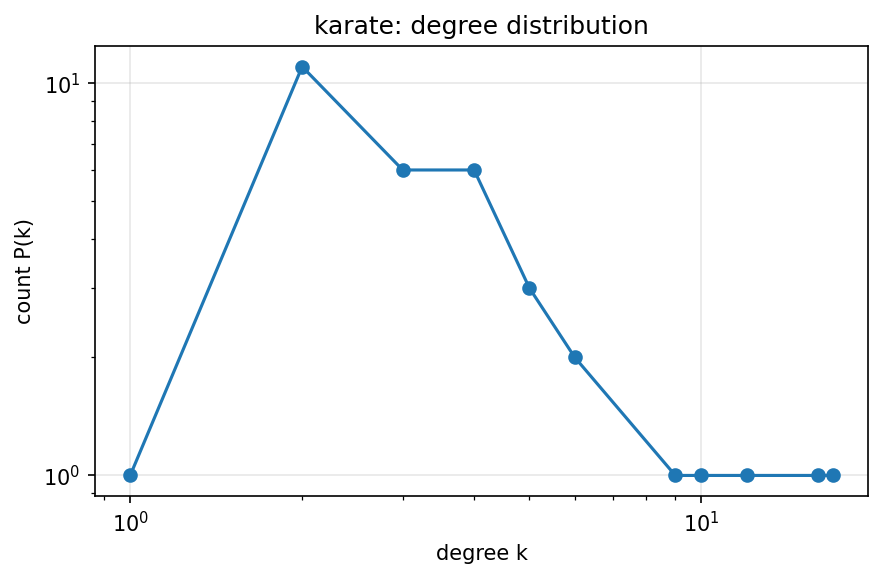
\includegraphics[width=0.7\textwidth]{06_karate_degree_dist.png}
\caption{Распределение степеней в карате-клубе (в логарифмических координатах)}
\label{fig:degdist}
\end{figure}

\subsection{Бенчмарк классических алгоритмов выделения сообществ}

Запущены восемь алгоритмов (Louvain, Louvain классический, Leiden, Label Propagation, Girvan-Newman, Fast Greedy, Walktrap) на всех шести датасетах с усреднением по трём прогонам на малых графах. Результаты для трёх характерных датасетов приведены в таблицах~\ref{tab:karate}, \ref{tab:football}, \ref{tab:email}.

\begin{table}[h]
\centering
\begin{tabular}{lrrrr}
\toprule
Алгоритм & NMI & ARI & $Q_{\mathrm{pred}}$ & $\hat k$ \\
\midrule
Louvain & 0.59 & 0.46 & 0.420 & 4 \\
Leiden & 0.59 & 0.46 & 0.420 & 4 \\
Label Propagation & 0.73 & 0.77 & 0.360 & 2 \\
Girvan-Newman & 0.49 & 0.39 & 0.401 & 5 \\
Fast Greedy & 0.56 & 0.57 & 0.381 & 3 \\
Walktrap & 0.49 & 0.32 & 0.353 & 5 \\
\bottomrule
\end{tabular}
\caption{Karate Club ($k^* = 2$)}
\label{tab:karate}
\end{table}

\begin{table}[h]
\centering
\begin{tabular}{lrrrr}
\toprule
Алгоритм & NMI & ARI & $Q_{\mathrm{pred}}$ & $\hat k$ \\
\midrule
Louvain & 0.85 & 0.70 & 0.597 & 9 \\
Leiden & 0.85 & 0.70 & 0.597 & 9 \\
Label Propagation & 0.90 & 0.82 & 0.600 & 10 \\
Walktrap & 0.89 & 0.82 & 0.603 & 10 \\
\bottomrule
\end{tabular}
\caption{Football ($k^* = 12$)}
\label{tab:football}
\end{table}

\begin{table}[h]
\centering
\begin{tabular}{lrrrr}
\toprule
Алгоритм & NMI & ARI & $Q_{\mathrm{pred}}$ & $\hat k$ \\
\midrule
Louvain & 0.57 & 0.29 & 0.417 & 7 \\
Leiden & 0.57 & 0.29 & 0.417 & 7 \\
Label Propagation & 0.00 & 0.00 & 0.000 & 1 \\
Walktrap & 0.57 & 0.19 & 0.347 & 110 \\
\bottomrule
\end{tabular}
\caption{email-Eu-core ($k^* = 42$)}
\label{tab:email}
\end{table}

Наглядное сравнение алгоритмов по NMI на всех датасетах представлено на рисунке~\ref{fig:nmi}.

\begin{figure}[h]
\centering
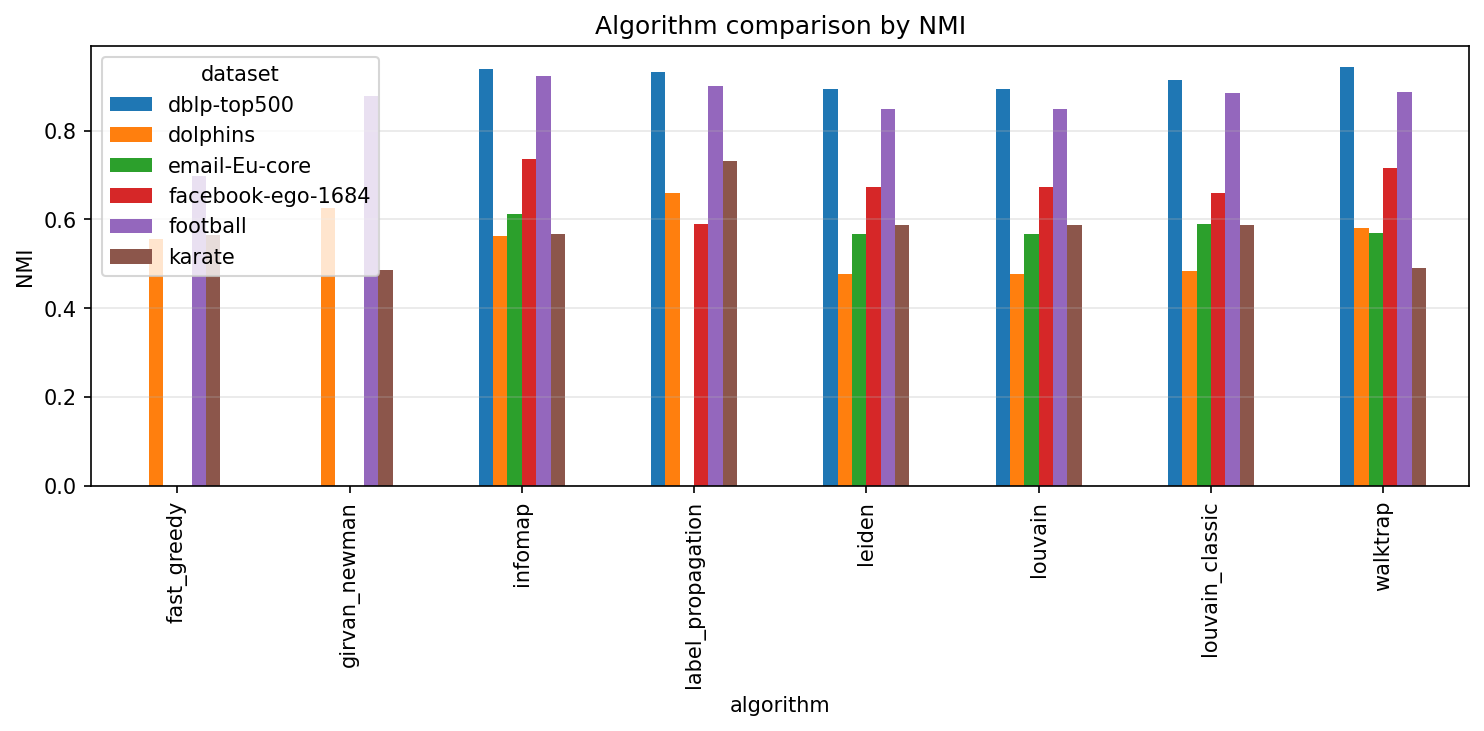
\includegraphics[width=0.95\textwidth]{02_compare_nmi.png}
\caption{Сравнение алгоритмов выделения сообществ по NMI}
\label{fig:nmi}
\end{figure}

\textbf{Интерпретация результатов.} Алгоритмы оптимизации модулярности (Louvain, Leiden) систематически переразбивают карате-клуб ($\hat k = 4$ при $k^* = 2$) и недоразбивают email-Eu-core ($\hat k = 7$ при $k^* = 42$). Это прямое проявление предел разрешения \cite{fortunato2007}. На плотном email-Eu-core с 42 классами Label Propagation коллапсирует в единственную метку ($\operatorname{NMI} = 0$), что согласуется с известным ограничением алгоритма \cite{raghavan2007}. Ни один алгоритм не доминирует во всех условиях: на Karate Club лучший- Label Propagation; на Football- Walktrap; на email-Eu-core- Walktrap.

Рисунок~\ref{fig:karate} визуализирует разбиение карате-клуба алгоритмом Leiden в сравнении с истинным разбиением.

\begin{figure}[h]
\centering
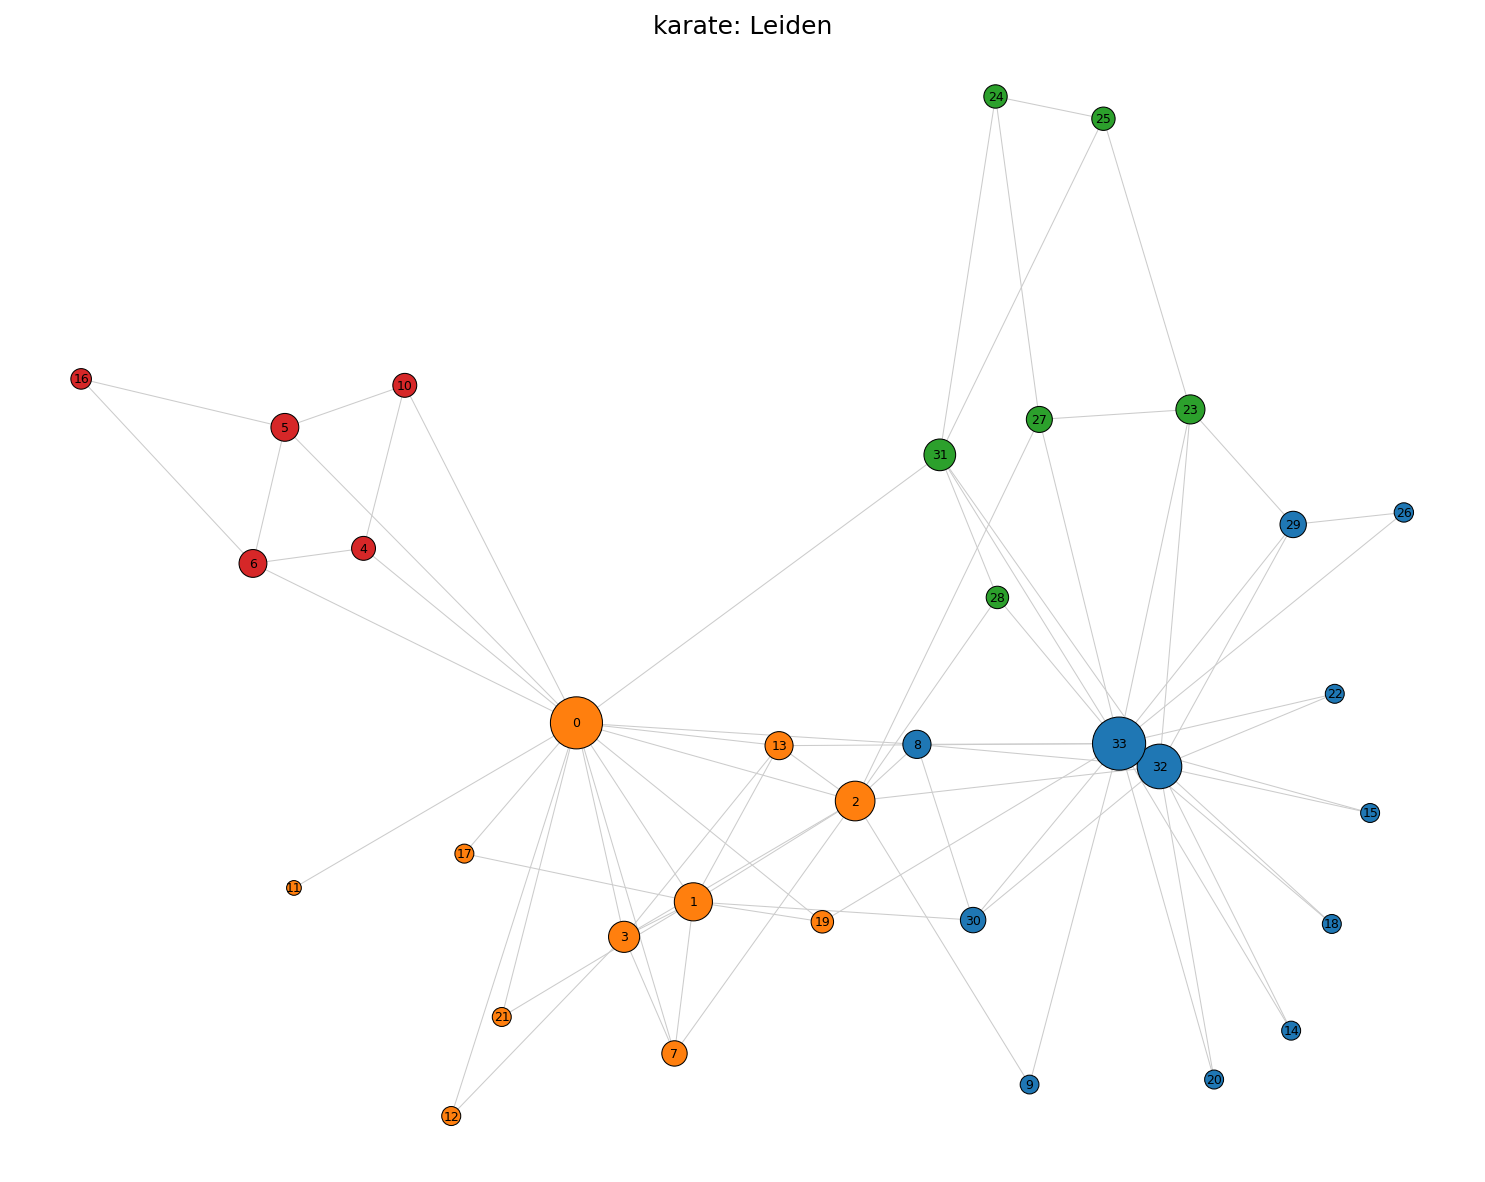
\includegraphics[width=0.48\textwidth]{06_karate_communities.png}\hfill
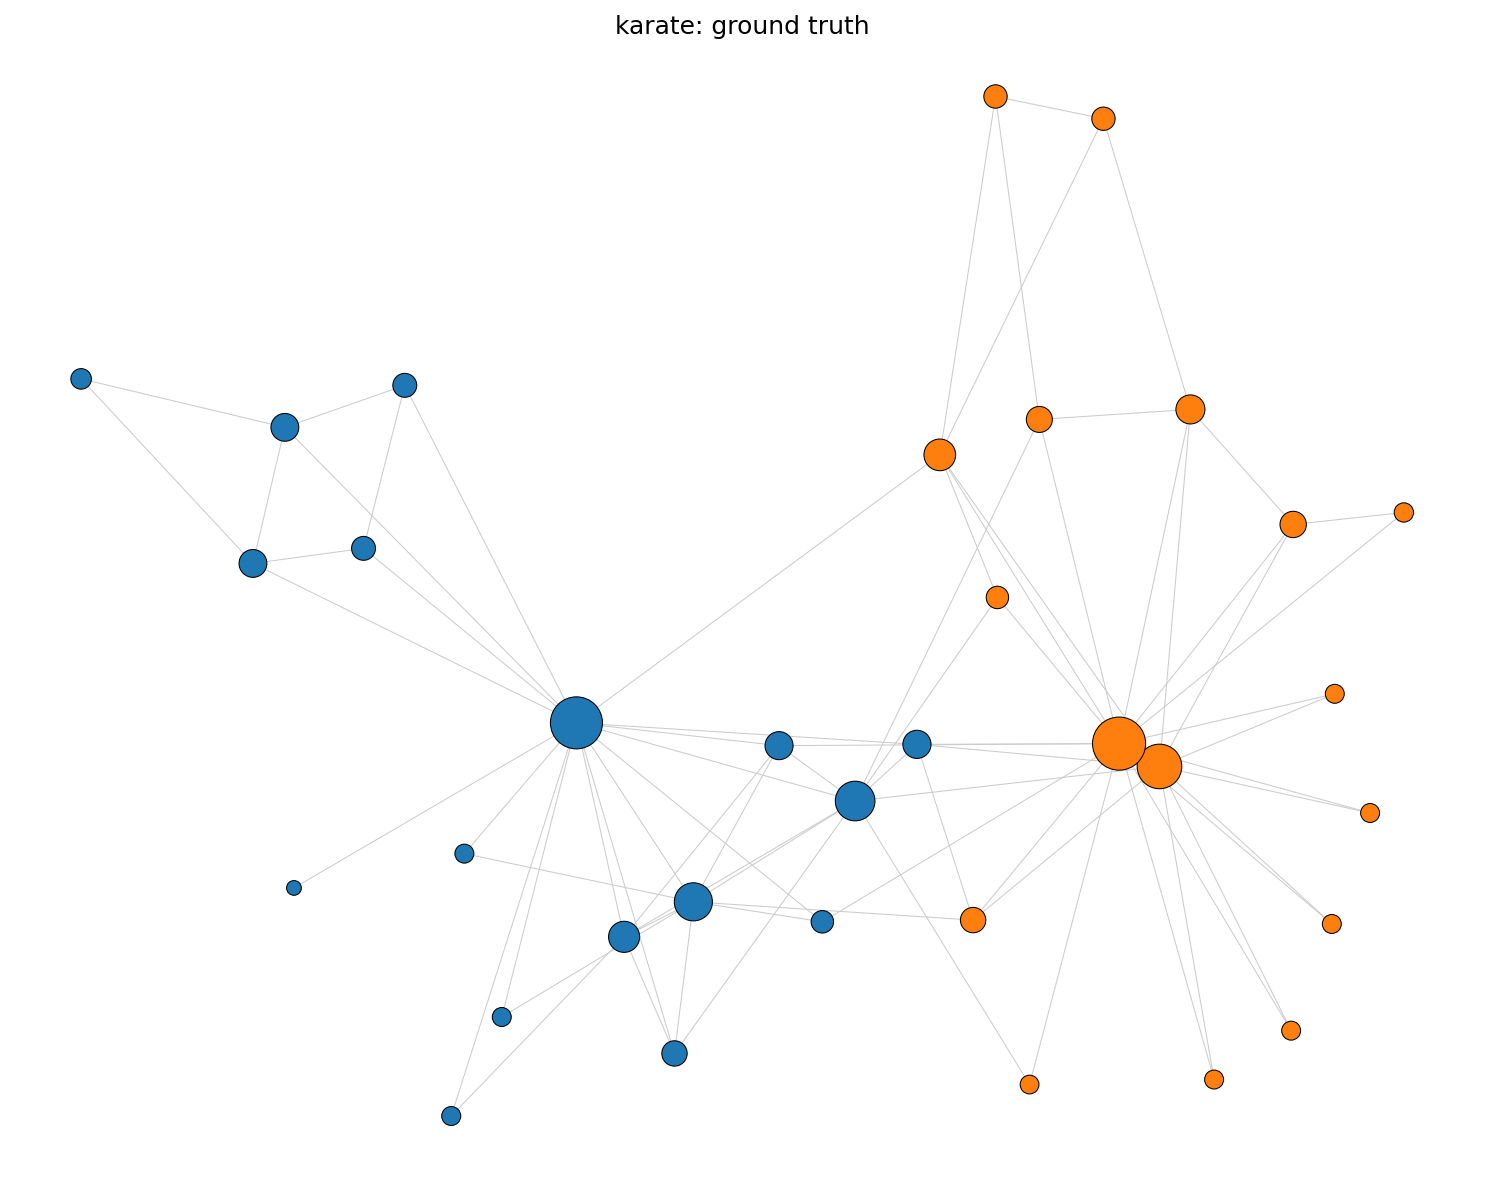
\includegraphics[width=0.48\textwidth]{06_karate_groundtruth.png}
\caption{Разбиение карате-клуба: слева- Leiden ($\hat k = 4$), справа- истинное разбиение ($k^* = 2$). Размер узла пропорционален PageRank}
\label{fig:karate}
\end{figure}

\subsection{Обучение графовых нейронных сетей}

GCN и GraphSAGE обучались в полу-управляемом режиме на стратифицированном разбиении 60/20/20. Гиперпараметры: hidden\_dim $= 64$, lr $= 0.01$, weight\_decay $= 5 \cdot 10^{-4}$, dropout $= 0.5$, до 500 эпох, ранняя остановка по val\_acc с patience $= 50$. Обученные модели сохранялись в каталог \texttt{models/}, что позволяет повторно получать те же предсказания без переобучения и обеспечивает воспроизводимость метрик.

\begin{table}[h]
\centering
\begin{tabular}{llrrrrr}
\toprule
Датасет & Модель & Train & Val & Test & NMI & ARI \\
\midrule
karate & GCN & 1.00 & 1.00 & 0.88 & 0.84 & 0.88 \\
karate & GraphSAGE & 1.00 & 1.00 & 0.88 & 0.84 & 0.88 \\
dolphins & GCN & 1.00 & 1.00 & 1.00 & 1.00 & 1.00 \\
dolphins & GraphSAGE & 1.00 & 1.00 & 1.00 & 1.00 & 1.00 \\
football & GCN & 0.88 & 0.87 & 0.87 & 0.89 & 0.83 \\
football & GraphSAGE & 0.90 & 0.87 & 0.87 & 0.90 & 0.82 \\
email-Eu-core & GCN & 0.84 & 0.83 & 0.78 & 0.82 & 0.75 \\
email-Eu-core & GraphSAGE & 0.98 & 0.81 & 0.81 & 0.90 & 0.87 \\
facebook-ego & GCN & 0.90 & 0.91 & 0.86 & 0.82 & 0.85 \\
facebook-ego & GraphSAGE & 0.98 & 0.90 & 0.84 & 0.88 & 0.91 \\
dblp-top500 & GCN & 1.00 & 1.00 & 0.98 & 0.99 & 0.99 \\
dblp-top500 & GraphSAGE & 1.00 & 1.00 & 0.99 & 1.00 & 1.00 \\
\bottomrule
\end{tabular}
\caption{Результаты обучения GCN и GraphSAGE на разбиении 60/20/20}
\label{tab:gnn}
\end{table}

\textbf{Интерпретация результатов.} Близость точности на тестовом множестве к точности на валидации (разность $\leq 0.03$ для GCN, до $0.17$ для GraphSAGE на email-Eu-core) свидетельствует об отсутствии переобучения. На самом сложном датасете (email-Eu-core, 42 класса) GraphSAGE даёт $\operatorname{NMI} = 0.90$ против $0.57$ у лучшего классического метода (Walktrap)- относительный прирост 58\,\%. На малых датасетах GCN и GraphSAGE дают сопоставимый результат: при малом $n$ обе модели сходятся к близкому решению.

\subsection{Выявление лидеров мнений}

Для каждого датасета вычислены пять метрик центральности и композитный ранг $R(v)$ (определение~2.10). Результаты для карате-клуба приведены в таблице~\ref{tab:leaders}.

\begin{table}[h]
\centering
\begin{tabular}{lrrrr}
\toprule
Узел & $\deg$ & $C_B$ & PR & $R(v)$ \\
\midrule
0 (Mr.\ Hi, тренер) & 16 & 231.07 & 0.097 & 1.50 \\
33 (John A., президент) & 17 & 160.55 & 0.101 & 1.75 \\
32 & 12 & 76.69 & 0.072 & 3.50 \\
2 & 10 & 75.85 & 0.057 & 3.50 \\
31 & 6 & 73.01 & 0.037 & 5.25 \\
\bottomrule
\end{tabular}
\caption{Лидеры мнений в карате-клубе \cite{zachary1977}}
\label{tab:leaders}
\end{table}

\textbf{Интерпретация.} Композитный ранг автоматически выделяет двух исторических лидеров карате-клуба- тренера Mr.\ Hi (узел~0) и президента John~A. (узел~33), вокруг которых произошёл реальный раскол в 1972~году. Это прямое эмпирическое подтверждение применимости теоретико-графового подхода к социометрии. На email-Eu-core лидером является узел~160 с $\deg = 345$ и $R(v) = 1.00$- сотрудник с максимальным числом email-контактов и наибольшим PageRank.

\subsection{Выявление изолированных групп}

В качестве предсказанного разбиения для расчёта conductance $\varphi(S)$ использовался результат Leiden \cite{traag2019}. Применены три эвристики: несвязные компоненты, сообщества с малым conductance, периферия по $k$-core.

\textbf{Интерпретация.} На карате-клубе обнаружены три низко-conductance сообщества ($\varphi \leq 0.143$) и одна периферийная вершина (coreness $= 1$). На сети футбола найдена клика-конференция размера~9 с внутренней плотностью $1.000$ и conductance $0.148$- конференция, играющая преимущественно внутри себя. На DBLP обнаружено сообщество размера~26 с conductance $0.002$ и плотностью $0.926$- типичная малая исследовательская группа, почти полностью изолированная от остального графа: conductance близок к нулю означает, что почти все рёбра группы- внутренние.

% ===========================================================================
% ЗАКЛЮЧЕНИЕ
% ===========================================================================
\section*{ЗАКЛЮЧЕНИЕ}
\addcontentsline{toc}{section}{ЗАКЛЮЧЕНИЕ}

В курсовом проекте решены все поставленные во введении задачи.

\textbf{1. Актуальность темы, история вопроса и обзор литературы.} Прослежено развитие методов анализа социальных графов от социограмм Морено \cite{moreno1934} (1934) к эре модулярности \cite{girvan2002,blondel2008,traag2019} (2002-2019) и к графовым нейронным сетям \cite{kipf2017,hamilton2017} (с 2017). Систематизированы три современных семейства методов: модулярность, случайные блуждания, нейронные сети.

\textbf{2. Математическая модель.} Дано строгое определение графа, моделей случайных графов (G(n, p), BA, WS), модулярности Ньюмана, метрик качества (NMI, AMI, ARI, accuracy) и центральности (degree, betweenness, closeness, eigenvector, PageRank), архитектур GCN и GraphSAGE.

\textbf{3. Программная реализация.} Реализован модуль бенчмарка с единым интерфейсом $f \colon G \to \mathbb{Z}^n$. GNN обучаются с корректным разделением вершин на обучающую, валидационную и тестовую выборки и сохранением модели в чекпоинт, что обеспечивает воспроизводимость результатов.

\textbf{4. Эмпирическое сравнение.} На шести датасетах разного размера установлено: алгоритмы модулярности страдают от предел разрешения \cite{fortunato2007}, Label Propagation \cite{raghavan2007} коллапсирует на плотных графах с большим числом классов, Walktrap \cite{pons2006} наиболее устойчивы среди классики. При наличии частичной разметки GraphSAGE \cite{hamilton2017} даёт $\operatorname{NMI} = 0.90$ на email-Eu-core против $0.57$ у лучшего классического метода- относительный прирост 58\,\%.

\textbf{5. Содержательные результаты.} Композитный ранг центральностей автоматически выделяет двух исторических лидеров карате-клуба, что подтверждает применимость подхода. Эвристики conductance и $k$-core обнаруживают изолированные структуры с ясной социальной интерпретацией: клики-конференции в Football, исследовательские группы в DBLP.

\textbf{Рекомендации.} Без разметки- использовать Leiden или Walktrap; при наличии разметки- GraphSAGE. Корректное использование обучающая/валидационная/тестовая выборки и чекпоинтов обязательно для воспроизводимости.

\textbf{Дальнейшие направления:} архитектуры GAT, GIN; временные графы; перекрывающиеся сообщества; применение к задачам обнаружения координированной дезинформации.

% ===========================================================================
% СПИСОК ИСТОЧНИКОВ
% ===========================================================================
\begin{thebibliography}{99}
\addcontentsline{toc}{section}{СПИСОК ИСПОЛЬЗОВАННЫХ ИСТОЧНИКОВ}

\bibitem{moreno1934}
Moreno, J.~L. Who Shall Survive? - Washington : Nervous and Mental Disease Publishing, 1934. - 440~p.

\bibitem{erdos1959}
Erdős, P., Rényi, A. On Random Graphs~I // Publicationes Mathematicae. - 1959. - Vol.~6. - P.~290-297.

\bibitem{zachary1977}
Zachary, W.~W. An information flow model for conflict and fission in small groups // Journal of Anthropological Research. - 1977. - Vol.~33, No.~4. - P.~452-473.

\bibitem{watts1998}
Watts, D.~J., Strogatz, S.~H. Collective dynamics of small-world networks // Nature. - 1998. - Vol.~393. - P.~440-442.

\bibitem{barabasi1999}
Barabási, A.-L., Albert, R. Emergence of scaling in random networks // Science. - 1999. - Vol.~286, No.~5439. - P.~509-512.

\bibitem{girvan2002}
Girvan, M., Newman, M.~E.~J. Community structure in social and biological networks // Proceedings of the National Academy of Sciences. - 2002. - Vol.~99, No.~12. - P.~7821-7826.

\bibitem{fortunato2007}
Fortunato, S., Barthélemy, M. Resolution limit in community detection // Proceedings of the National Academy of Sciences. - 2007. - Vol.~104, No.~1. - P.~36-41.

\bibitem{raghavan2007}
Raghavan, U.~N., Albert, R., Kumara, S. Near linear time algorithm to detect community structures in large-scale networks // Physical Review~E. - 2007. - Vol.~76, No.~3. - P.~036106.

\bibitem{blondel2008}
Blondel, V.~D., Guillaume, J.-L., Lambiotte, R., Lefebvre, E. Fast unfolding of communities in large networks // Journal of Statistical Mechanics: Theory and Experiment. - 2008. - No.~10. - P10008.

\bibitem{pons2006}
Pons, P., Latapy, M. Computing communities in large networks using random walks // Journal of Graph Algorithms and Applications. - 2006. - Vol.~10, No.~2. - P.~191-218.

\bibitem{brandes2008}
Brandes, U., Delling, D., Gaertler, M. et al. On modularity clustering // IEEE Transactions on Knowledge and Data Engineering. - 2008. - Vol.~20, No.~2. - P.~172-188.

\bibitem{newman2010}
Newman, M.~E.~J. Networks: An Introduction. - Oxford : Oxford University Press, 2010. - 720~p.

\bibitem{diestel2017}
Diestel, R. Graph Theory. - 5th ed. - Heidelberg : Springer, 2017. - 428~p.

\bibitem{defferrard2016}
Defferrard, M., Bresson, X., Vandergheynst, P. Convolutional neural networks on graphs with fast localized spectral filtering // Advances in Neural Information Processing Systems. - 2016. - P.~3844-3852.

\bibitem{kipf2017}
Kipf, T.~N., Welling, M. Semi-supervised classification with graph convolutional networks // Proceedings of ICLR. - 2017. - \texttt{arXiv:1609.02907}.

\bibitem{hamilton2017}
Hamilton, W.~L., Ying, R., Leskovec, J. Inductive representation learning on large graphs // Advances in Neural Information Processing Systems. - 2017. - P.~1024-1034.

\bibitem{traag2019}
Traag, V.~A., Waltman, L., van Eck, N.~J. From Louvain to Leiden: guaranteeing well-connected communities // Scientific Reports. - 2019. - Vol.~9. - Article~5233.

\bibitem{kingma2015}
Kingma, D.~P., Ba, J. Adam: A method for stochastic optimization // Proceedings of ICLR. - 2015. - \texttt{arXiv:1412.6980}.

\bibitem{snap}
Leskovec, J., Krevl, A. SNAP Datasets : Stanford Large Network Dataset Collection [Электронный ресурс]. - Режим доступа: \url{https://snap.stanford.edu/data}. - Дата доступа: 21.05.2026.

\end{thebibliography}

\end{document}
